\documentclass[a4paper,12pt]{article}
\usepackage[latin1]{inputenc}
\usepackage[spanish]{babel}
\usepackage{bm}
\usepackage{graphicx}
\usepackage{amsmath}
\setlength{\textheight}{235mm}
\setlength{\textwidth}{168mm}
\setlength{\oddsidemargin}{0pt}
\pagestyle{empty}
\begin{document}
\mbox{}\vspace*{-45mm}

{\centering
{\small\sc Escuela T�cnica Superior de Ingenieros de Caminos, Canales y
Puertos (Madrid)}\\*[4mm]
{\Large\bf M�todo de los Elementos Finitos (Curso 19-20)}\\*[4mm]
Ejercicio 5: Tecnolog�a de elementos \\*[4mm]

}

\vspace{3mm}

%%%%%
\parbox{0.50\textwidth}{
Se considera una l�mina cil�ndrica de radio medio $R=300$,
longitud $L=600$ y espesor $t=3$, cuyo material es el�stico lineal con
propiedades mec�nicas $E=300$ y $\nu=0.3$. Los extremos del cilindro est�n
fijos y en dos puntos diametralmente
opuestos de la secci�n transversal media est�n aplicadas sendas cargas radiales
de compresi�n de valor $P=1.0$ cada una de ellas.
Para la discretizaci�n se tendr�n en cuenta las condiciones de
simetr�a existentes, y se utilizar� una discretizaci�n de $32 \times 32$,
elementos en direcci�n meridional y circunferencial, y $1$ elementos en el
espesor. Las
formulaciones a considerar son hexaedros de $8$ nodos con formulaci�n
isopar�metrica, con formulaci�n mixta y con deformaciones mejoradas supuestas.
}\hfill
\parbox{0.50\textwidth}{ \hfill
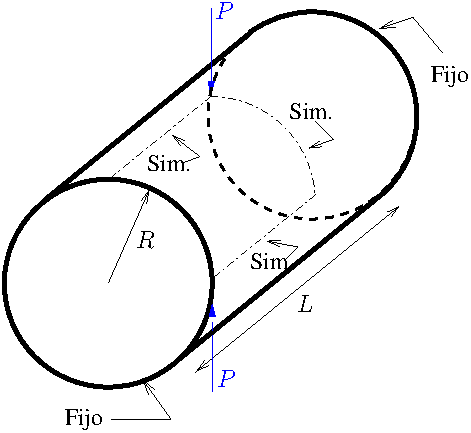
\includegraphics[width=0.45\textwidth]{pinched}
}
\end{document}
